\documentclass[a4paper]{article}
\usepackage[utf8]{inputenc}
\usepackage[english]{babel}
\usepackage[T1]{fontenc}
\usepackage{amsmath,amssymb}
\usepackage{mathtools}
\usepackage{color}
\usepackage{graphics}
%\usepackage{amssymb}

\author{Giovanna Fancello, Olivier Cailloux, Alexis Tsoukiàs}
\title{Tourists'preferences ...}
\pagenumbering{arabic}
\begin{document}
\maketitle
\begin{abstract}
abstract

abstract

abstract

abstract
\end{abstract}

\tableofcontents

\section{Introduction}
\begin{itemize}
   \item [-]principal aim of the paper: to define public policies legitimated and that take account of people values and diversities.
   \item [-]the tourist as one of the population in the city
   \item [-]the possibility to access to some urban opportunity in order to improve their urban-quality of life (in a capability theory point of view)
 \end{itemize}

\textbf{Main Objective.}
The aim of this work is to define a method able to inspect values in space as regard to people variety in order to define public policies legitimated by different categories of people, policies that take account of people values and diversities. The purpose is to personalize the territorial offer of opportunities (to do or be in space) in respect to people values, preferences and needs. Especially, the research inquires how to collect and to analyse these features in order to be useful for the policy cycle and how to synthesize them in space considering the differences among individual values. In order to do this, we propose a replicable method able to inspect values that individuals give to different spaces.

Values in space can be learned by behaviours or declared preferences. 
In this study we use both type of data and experiment different methods and a replicable procedure for the analysis of preferences of tourists in the Alghero territory. Among the methods we used: multiple regression model; additive value function models (UTA family); multi task regression model;...

In the following paragraphs we first describe the problem, than we explore the literature in order to select the methods more suitable for our analysis. In the following section we explain the final method proposing an application to the case study. Finally, some policy analytics recommendation are given.


\section{The problem. Alghero case study}
 Alghero is a city in the north east coast of the Sardinian Region (ITALY), characterized by an economic dependance from the touristic season for the development of the territory. This economic development can bring to positive but also negative consequences, given by that temporal economy that risk to influence the territorial development, as well as to the services and opportunities that has to be strategically improved in order to meet the needs of different population that live the city (CITARE MARTINOTTI). The activities undertaken by the people varies, among others, according to individual characteristics and interests \cite{Kellner2016}, to spatial distribution of urban and territorial activities and to quality of the accessibility in the city \cite{Blecic2015a}.
Therefore, a strategic public policy should consider, among others, needs and preferences of tourist population in order to strategically improve the quality of life of the territory. Especially, a policy attentive to different people values can help in developing personal urban capabilities with the improvement of that urban opportunities that are most valued by tourist population (what people value \cite{Sen1999}.

 In order to help policy makers in define new public policies, this work  aims to define groups of people with common values of the space. A purpose different from the statistical analysis of people in respect to the correspondent tourist socio-professional class and behaviours. What we try to do is a clusterization of population with similar values and interests in the city. This allows to define territorial development policies focused to specific tourist population and to improve the urban opportunities of the territory. Moreover, this analysis allows to define and to propose to different populations new doings and beings (urban capabilities) that they didn't already knows. Similar people in the same territory have similar urban capabilities, but may be they are not interested in them in the same manner, as they didn't value all these capabilities as important. In this work we want to bring to light similar values in space, similar capabilities that can be offered of people of the same group.


\subsection{The survey}
We analyse the tourist population in Alghero during the 2014 touristic "low season" (October-November), considering that Alghero's peek period is the summer season with highest tourist concentration between July and September. Data collection was carried out in this period because we want to catch urban limits and opportunities in a period of reduction of urban activities and not bathing season and have significant information for design a public policy aimed to deseasonalize this trend. These data was collected for the project \textcolor{red}{XXX, lo inseriamo nel testo o in nota?}.
Two type of data were collected in the survey: interviews to inspect expectations and degree of satisfaction and GPS movement tracking to explore tourists' movements in the territory.

Especially, we dispose of 75 questionnaires representing \textbf{225 tourists $T$} described by a \textbf{set of attributes $A$}
\begin{equation}
A=\{gender,age,country,level of study,profession,willingness to pay\}
\end{equation}
We know the \textbf{tourists' paths} in the territory, in a space described by \textbf{Coordinates} and \textbf{Time}.
Let $S$ denote the set of possible coordinates and $\tau$ the set of possible times.  A path is a set of points $P \subseteq S \times \tau$.\\
Finally we define a set of \textbf{Categories of places} $C \in S$ that a tourist can choose in Alghero city.

In order to have coordinates divided in categories of space we did a spatial classification analysis of  coordinates data (Figure \ref{10places}). Especially we:
\begin{enumerate}
\item \textbf{Split the space} Subdivide the territory in different places $p$.
\item \textbf{Classify spaces.} Classify each place $p$ in a Category $c$
\item \textbf{Count the time.} For each tourists' path we analyse the time spent for any category of place $c$.For each $t$ we analyse how much time the he spent in it $x^t (c)$. The time spent in any category is given by the sum of the different ranges of time in this category of place $x^t (c_v)$. We consider that each tourist has 15 hours to spend in a day.
\end{enumerate}

\begin{figure}
  \centering
    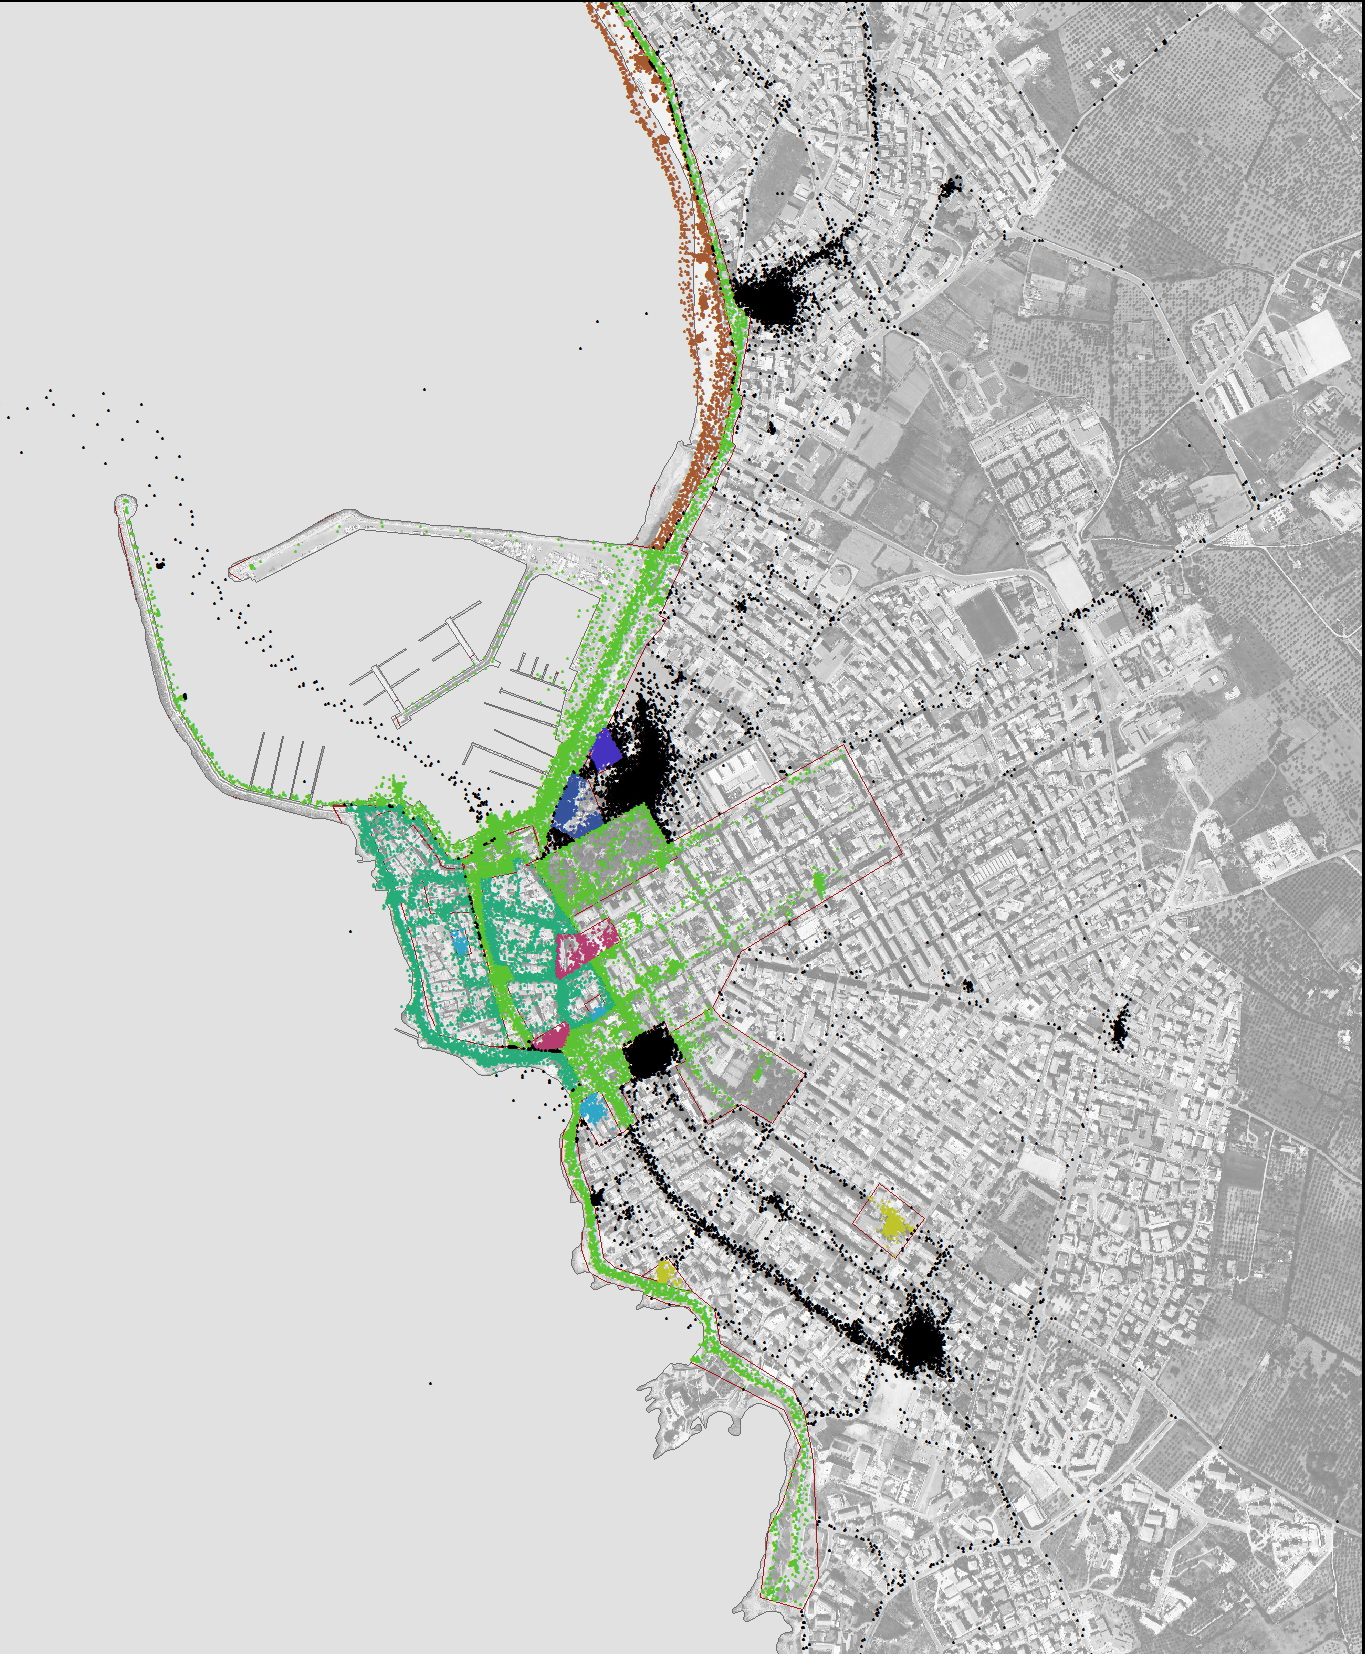
\includegraphics[width=\textwidth]{10places}\\
  \caption{Classification of paths in respect to categories of places}\label{10places}
\end{figure}


Let $C=\{c_1, \ldots, c_7\}$ denote the set of categories of places.

\begin{table}[h]
\begin{tabular}{ll}
\hline
\textbf{Categories of places}&\textbf{Places}\\
\hline
\parbox{5cm}{Environmental elements (local)}&\parbox{6cm}{Lido, M. Pia, \dots}\\
\parbox{5cm}{Environmental elements (territorial)}&\parbox{6cm}{Grotte di Nettuno, Punta Giglio, Spiaggia del Lazzaretto, \dots}\\
\parbox{5cm}{Historical and archaeological elements (local)}&\parbox{6cm}{Cattedrale,Bastioni,Historical centre, \dots}\\
\parbox{5cm}{Historical and archaeological elements (territorial)}&\parbox{6cm}{Fertilia, Castelsardo, Stintino, nuraghe Palmavera, \dots}\\
\parbox{5cm}{Cultural Elements}&\parbox{6cm}{Theater, Cinema, Museum, \dots}\\
\parbox{5cm}{Food services}&\parbox{6cm}{Restaurants, Market,\dots}\\
\parbox{5cm}{Leisure}&\parbox{6cm}{Waterfront, Public Gardens, Harbor, \dots}\\
\parbox{5cm}{Other}&\parbox{6cm}{Stay in the Hotel, friends' home, Route from one place to another, \dots}\\
\hline
\end{tabular}

\caption{\textbf{Categories of places}}\
\label{Table1}
\end{table}

We call $i^t \in {\mathbb{R}^+}$ the total number of seconds a tourist $t$ has spent on his trip in the different categories of places.

Starting with these considerations:


\newtheorem{mydef}{Definition}
\begin{mydef}
A \textbf{vector path} $x: C \rightarrow R^+$ is a function that maps each category of places to a number of seconds.We associate to each tourist $t \in T $ a vector path $x^t$. Let $X={\mathbb{R}^+}^C$ denote the set of all possible vector paths.
\end{mydef}

Among all the vector paths the tourist chose a path in respect to his preferences and values.

\begin{mydef}
A \textbf{preference relation} is a binary relation over the set of possible vector paths $S \subseteq X \times X $,.
\end{mydef}

 In detail, a preference relation is given when the tourist can freely choose a path to another in respect to his individual characteristics (age, gender,\dots) and to his personal (income,\dots) and spatial resources (means of transport, \dots) \cite{Sen1999}.

  Considering this, our objective is to associate to each tourist $t \in T$ a preference relation $S_t$ which represents, according to our model, the way the tourist evaluates the possible paths in the Alghero territory, i.e. the way the tourist values the space. This preference relation can also reveal important elements for the design of new paths in respect to the "demand? (like marketing?)" of the tourist population in Alghero. Let $X^t {\subseteq}X$ denote the set of all vector paths that can be freely  chosen by $t$.


Finally, we know the \textbf{tourist declared preferences} (why they choose to stay in Alghero and what they want to do). The criteria the tourists used to choose to visit Alghero that are ordered by importance with an evaluation scale. Let's have for each tourists' criteria $zt \in Zt$ a value $n \in \xi$ with $\xi\{1,2,3,4,5\}$
\begin{equation}
\begin{split}
Zt&=n\{Economy,Environment,Weather,Food,Culture,Recreation,\\
&Entertainment,Study,Work,Relax,Friends and relatives,others\}
\end{split}
\end{equation}


\subsection{Synthesis of Data}
In synthesis the set of data is given by the:
\begin{description}
	\item[$T$] Set of tourists ($t$ a tourist)
	\item[$Z$] Set of aspects on which tourist has declared a degree of interest ($Zt$)
	\item[$d^t: Z \rightarrow \{1, 2, 3, 4, 5\}$] A function such that $d^t(z) \in \{1, 2, 3, 4, 5\}$ indicates, for tourist $t \in T$ and aspect $z \in Z$, the degree of interest on aspect $z$ as declared by $t$
	\item[$i^t \in {\mathbb{R}^+}$] Intensity corresponding to $t$: the total number of seconds tourist $t$ has spent on his trip in the different categories of space.
	\item[$C_V$] The categories of places in Alghero \emph{that can be visited}, thus \emph{including} staying home.
    \item[$x^t: C_V \rightarrow {\mathbb{R}^+}$] The vector path chosen by tourist $t$ that associates a number of seconds to each category of place. By definition, $\sum_{c \in C_V} x^t(c) = i^t$.
       \end{description}
\textcolor {red}{$x^t$ E' l'insieme DI PUNTI CHE FORMANO IL PERCORSO FATTO DA UN TURISTA IN UNA DETERMINATA CATEGORIA DI LUOGO, iN REALTà IL PERCORSO è DIVERSO, NOI ABBIAMO PRESO TUTTI I PUNTI INTERNI AD UN LUOGO}


\subsection{A simple goal}
 DA PROPOSTA DI OLIVIER


Our goal is to predict $x^t$ given $d^t$ and an intensity: a number of seconds that indicates how long the tourist intends to visit for. We are allowed to use $T_1 \subseteq T$ as training data, and must use $T_2 \subseteq T$ as test data. Given a predictor $P: \{1, 2, 3, 4, 5\}^Z \times {\mathbb{R}^+} \rightarrow {\mathbb{R}^+}^{C_V}$, the quality of $P$ is the sum, on the test data, of the distance, using L2 norm, between the prediction and the real path: quality of $P$ = $\sum_{t \in T_2} \|P(d^t, i^t) $-$ x^t\|$.

Here below we list a few possible ways of building predictors, starting from the simplest ones:

\begin{itemize}
    \item \textbf{central prediction} We compute the centre (using L2) of $(x^t)_{t \in T_1}$ and constantly predict this.
    \item\textbf{Unlinked regression} Build some regression model between ${\{1, 2, 3, 4, 5\}}^Z \times {\mathbb{R}^+}$ and each dimension of ${\mathbb{R}^+}^{C_V}$, separately.
    \item \textbf{Multi-task Regression}Build some regression model between ${\{1, 2, 3, 4, 5\}}^Z \times {\mathbb{R}^+}$ and ${\mathbb{R}^+}^{C_V}$.
 \textcolor{red}{WORK IN PROGRESS WITH ELASTICNET MIXING PARAMETERS}
    \item \textbf{UTA+ Method}
    \item \textbf{Learned transformation}Same idea as Transformed space, but we learn the partial value functions using $T_1$.
    \item \textbf{Guided regression}Same idea but we (somehow) use knowledge about the link between $Z$ and $C_V$.
    \item \textbf{Transformed space}We fix (a priori) a set of partial value functions $u_c: {\mathbb{R}^+} \rightarrow [0, 1]$, one for each category of place. The vector $(u_c \circ x^t): C_V \rightarrow [0, 1]$ represents the values associated by tourist $t$, given its path, to each category of places. We learn a regression model (using normal or guided regression) between ${\{1, 2, 3, 4, 5\}}^Z \times {\mathbb{R}^+}$ and latent weights $w^t$, in order to maximize $w^t \cdot (u_c \circ x^t)$, the value of $x^t$.
     \item \textbf{More ideas}See article Siskos. See utilitaristic regression from Eyke.
\end{itemize}


\section{Background}
In order to define a method to analyse values in space for different touristic populations we can use several methods. In literature we can distinguish almost two fields of research that interested in our research.
\begin{itemize}
    \item {Analysis of tourist behaviours in space}
    \item {Analysis of people values (in respect to declared preferences or judgments)}
\end{itemize}
These two fields have to be combined for our research problem, especially we can consider the first analysis of tourist behaviour as the method to have data  for the analysis of people values.


\subsection{Tourist behaviours in space}
The most common way to study tourists’ behaviours in time and space are various methods of diary (re)construction \cite{Shoval2014}. New possibilities have arisen by the development of automated tracking, above all the satellite-based (e.g. GPS) technologies for automatic position tracking with high time and spatial resolution.
Even if methods for surveying and analysing spatio-temporal behaviour are, of course, becoming highly developed in transportation research and in social sciences in general, comparatively little attention was being paid to the spatial and temporal behaviour of tourists, and systematic studies taking advantage of the technological developments offered by the high precision position tracking are still relatively few \cite{Shoval2007};\cite{Shoval2014}.
In recent years scholars have started to break ground in this specific domain of applied research, experimenting and exploring advantages and disadvantages of satellite-based positioning technologies for the study of tourists’ spatio-temporal behaviours \cite{Shoval2010}.
Different methods have been reported for tracking tourist spatio-temporal behaviour \cite{Kellner2016}:
\begin{itemize}
    \item direct observation of tourists’ activities, with interviews or remote observations;
    \item {time-space budget techniques \cite{Pearce1988} which analyse tourists’ activities within destina-tions by using diaries, questionnaires and interviews;}
    \item {video-based tracking analysis, used to track tourists movements through video footages;}
    \item {smartphones with apps using positioning systems;}
    \item {specialized GPS tracking devices}
    \item {land-based tracking systems that collect data thanks to radio technology.}
\end{itemize}
Many studies report observations on a small scale, focusing on particular urban areas or activities that have a clearly defined entry and exit point, such as natural parks or historical centres \cite{Shoval2014}. Also many urban contexts have been analysed, among which Rome \cite{Calabrese2006}, Lago del Garda \cite{Bruno2010}, Canberra and Sydney \cite{Edwards2009}, Salzburg \cite{Kellner2016}. On the other side, there are studies that attempt to analyse tourist behaviours at very large scale (e.g. on the national scale, by using mobile phones data \cite{Ahas2007}.
Different statistical and visualisation techniques may be employed to analyse and represent such spatial data. Frequently spatial temporal data are used only to de-scribe the tourists track in maps. Sometimes these spatial maps are combined further information collected through questionnaires. This allows to link spatial temporal behaviour to a specific tourist category of population. Furthermore, of interest are studies trying to predict visitors whereabouts, how long they will stay in a place, or carry out a specific activity \cite{Chhetri2010}.


\subsection{People values and preferences}
Value theory





\subsubsection{Unlinked regression}
We start building predictors with the multiple regression model.

The definition of $x^t$ depends on the number of seconds in a category of place(\textcolor{red}{HO BISOGNO DI SPIEGARE IL PROBLEMA DAL PUNTO DI VSTA FORMALE?}).  This means that we have two dependent elements that are influenced  by the preferences of people ($d^t$). We cannot use a standard multiple linear regression model, for this reason, in order to directly predict $x^t$, we develop an unlinked  multiple regression model aimed to investigate the relation among the different elements separately.

Especially, we develop a multiple regression model between ${\{1, 2, 3, 4, 5\}}^Z \times {\mathbb{R}^+}$ and each dimension of ${\mathbb{R}^+}^{C_V}$, separately.
Results (see Table \ref{Table1}) show low relations between the dependent variable and the independents ones. For example, the regression model between  ${\{1, 2, 3, 4, 5\}}^Z \times {\mathbb{R}^+}$ and ${\mathbb{R}^+}^{EnvLocal}$ shows a R-squared of 0.2397 and a low significance of  independent variables (the $t test$).

We also develop a regression model isolating the set of aspects $z \in Z$ that have much more significance, but also in this case we obtain low significance values.

This means that this method is not able to building predictors with this type of data.

\begin{table}[ht]
\centering
\begin{tabular}{rrrrrr}
  \hline
 & Estimate & Std. Error & t value & Pr($>$$|$t$|$)& signif. \\
  \hline
(Intercept) & 7226.3916 & 3559.1948 & 2.03 & 0.0472&* \\
  cost & 151.3463 & 484.6296 & 0.31 & 0.7560 \\
  environment & -803.0865 & 471.5940 & -1.70 & 0.0942 \\
  weather & -200.6880 & 598.4546 & -0.34 & 0.7386 \\
  health & 946.1080 & 710.4019 & 1.33 & 0.1884 \\
  food & -1581.7536 & 589.8456 & -2.68 & 0.0097&** \\
  events & 1825.5161 & 744.7139 & 2.45 & 0.0174&* \\
  sport & 128.9466 & 614.9811 & 0.21 & 0.8347 \\
  fun & -165.3657 & 848.8539 & -0.19 & 0.8463 \\
  study & -310.8244 & 946.6043 & -0.33 & 0.7439 \\
  work & -1562.5287 & 715.1637 & -2.18 & 0.0332&* \\
  relax & -135.9579 & 500.6331 & -0.27 & 0.7870 \\
  family & 714.5345 & 552.7549 & 1.29 & 0.2015 \\
   \hline
 \end{tabular}
\begin{tabular}{rr}
Signif. codes&  $0 *** 0.001 ** 0.01 * 0.05 . 0.1   1$\\

Residual standard error& 4922 on 55 degrees of freedom\\

Multiple R-squared&  0.2397,    Adjusted R-squared:  0.07384\\

F-statistic& 1.445 on 12 and 55 DF,  p-value: 0.1742\\
   \hline
\end{tabular}
\caption{\textbf{Unlinked regression. Example by Environmental Local places}}\
\label{Table1}
\end{table}

\section{UTA+ Method}
As second method we present a multicriteria model that combines preference learning methods with the unsupervised machine learning in order to define the best territorial offer for each category of people. It is a sort of territorial marketing aimed to satisfy what people value as important to do \cite{Sen1999} in the territory.  What we want to inspect is not only what people do in respect to different needs and values, but to understand which are the set of things that people can do in the territory starting from their preferences and needs.


The model proposed is composed of different phases:
\begin{enumerate}
\item \textbf{data collection} NON SO SE INSERIRLO DI NUOVO QUI
\item \textbf{Multicriteria analysis of preferences}. In order to do this we use the UTA+ algorithm.
\item \textbf{Selection of relevant factors for personalization}.
\subitem Cluster analysis of the utility function
\subitem Rough set analysis
\item \textbf{Cluster analysis}. Cluster analysis of the results to define the different profiles of tourists
\item \textbf{Recommendation}
\end{enumerate}

\begin{figure} [ht]
  \centering
  % Requires \usepackage{graphicx}
  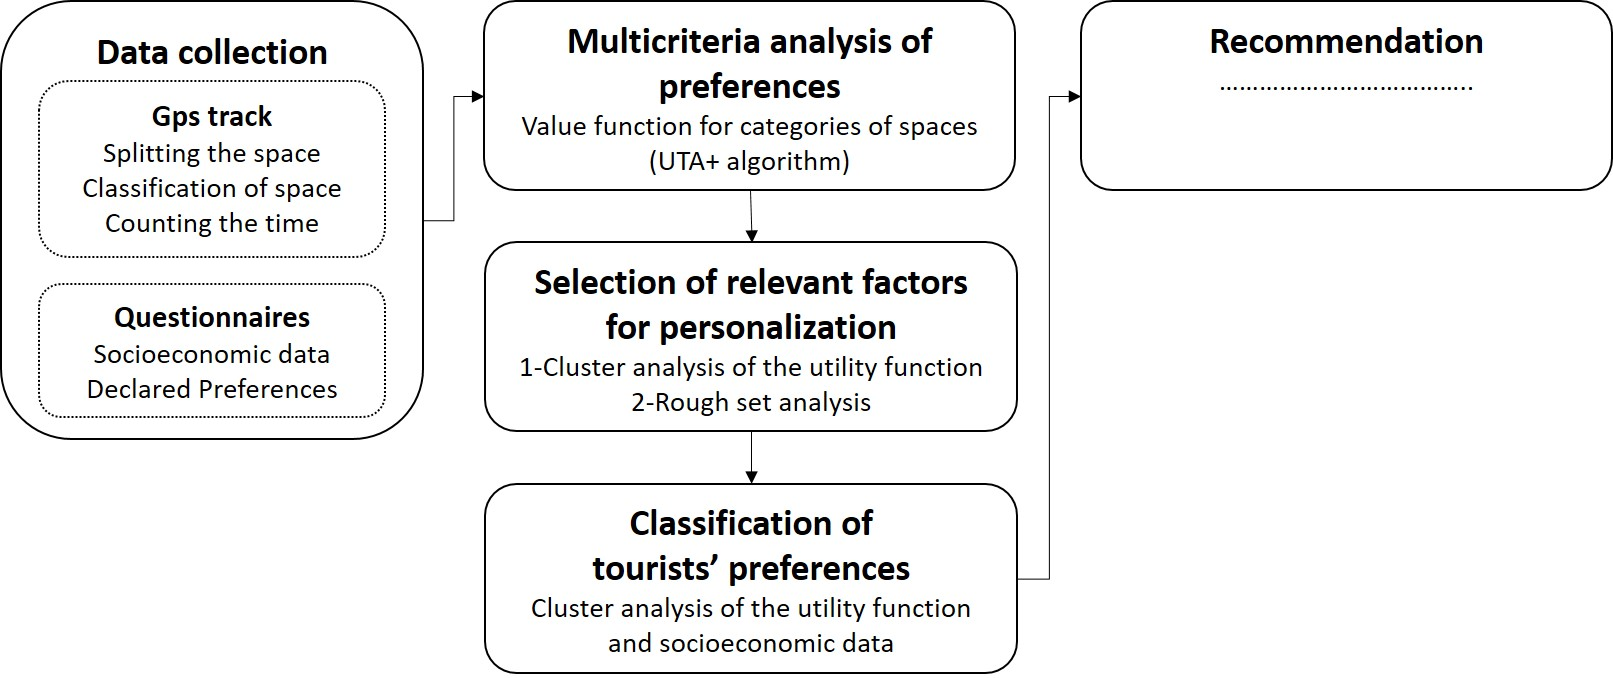
\includegraphics[width=\textwidth]{schema}\\
  \caption{Schema}\label{test}
\end{figure}


\subsection {Multicriteria analysis of preferences}
We consider that each tourist is a decision maker that needs an aid in order to understand his priorities and values in terms of what he can do in the Alghero territory.
To model this problem and define tourists' values we use the UTA algorithm.
UTA  was originally proposed by E.Jacquet-Lagraze and J.Siskos in 1982 \cite{Jacquet-Lagreze1982}. Especially, we use an implementation of the UTA method, the UTA+ algorithm \cite{kostkowski1996uta+}. This method solves problems of multicriteria choice and ranking on a set $A$ of alternatives.

\textcolor{red}{Spiego in geneale come funziona UTA?}
%The method can be used to solve the problems of multicriteria choice and ranking on a set A of alternatives. It constructs an additive utility function from a preference weak order defined by the user on a subset A' of reference alternatives. The construction, based on a principle of ordinal regression, consists of solving a small LP problem. The software proposes marginal utility functions in piecewise linear form as compatible as possible with the given weak order. It allows the user to modify interactively the marginal utility functions within limits following from a sensitivity analysis of the ordinal regression problem. For these modifications, the user is helped by a friendly graphical interface.It allows the user to modify interactively the marginal value functions within limits following from a sensitivity analysis of the formulated ordinal regression problem. During all these modifications, a friendly graphical interface helps the DM to reach an accepted preference model

Utility function can express user's preferences in respect to a set of alternatives. The UTA+ method consents to give a value of each alternative starting from a ranking of alternatives. The ranking is a weak order that uses the preference (P) and indifference (I) relations only among the reference alternatives.


We represent preference relations $S$ using additive value functions. Let $u^t$ denote the value function of tourist $t$. We define $S_t$ from  $u^t$ as follows:
\begin{equation}
(x_1,x_2) \in S_t \text { iff } u^t(x_1) \geq u^t(x_2).
\end{equation}

Our objective is thus to obtain $u^t$ from the path data.

We assume that $u^t$ can be represented as a weighted sum  of partial value functions:
\begin{equation}
u^t(x) = \sum_{c \in C} u_c(x_c) w^t_c,
\end{equation}
where $w^t \in [0,1]$ represents the weight that the tourist $t$ gives to the category of place $c$.

We assume for now that the partial value functions $\{u_c\}$ and the weights may depend on people values and are different for each tourist $t$.

Given a category $c \in C$, we define a partial value function $u_c:{\mathbb{R}^+} \rightarrow [0,1]$. The number $u_c(x_c)$ represents the value we assume the tourist gives to spending $x_c$ seconds in the category $c$, not taking into account the partial weight $w^t_c$.

We define each $u_c$ as a two linear pieces increasing function determined by the UTA method.

From now we know just the behaviours of each tourists $t$ and their declared preferences. In order to learn the set of tourists' preferences we consider the relation among the path chosen by the tourist and a set of \textbf{outstanding paths}. The outstanding paths are defined by a combination of categories of places $C$ and time $\tau$ they ideally spend in (with a maximum of 15 hours of visit). A tourist's preference is verified if the tourist $t$ prefers a path internal to his choice set $x_1 \in X^t$ in respect to another $x_2 \in X^t$.
\begin{mydef}
We define an outstanding path as a path that a tourist can freely choose in respect to his personal characteristics and spatial and personal resources (\textcolor{red}{TO BE COMPLETED} \dots).
\end{mydef}
We define two possible set of outstanding paths that are valid for all tourists:
                                            \begin{itemize}
                                                \item \textbf{Hard set}: all the tourist paths can be considered as outstanding paths. This means that a tourist $t$ prefers his path to all the other tourists' paths. But, as each tourist has his personal set of possible paths (in a capability framework), it is possible that $X^{t_1}\cap X^{t_2}$ or that $X^{t_1}\neq X^{t_2}$.
                                                    \subitem {-} \textcolor{red}{but not all the people has the same characteristics and the same resources, so we need to define different outstanding paths.}
                                                \item \textbf{Soft set}: a set of outstanding paths (see Table  \ref{Table2}), not expensive and reachable on foot. This permits to consider a sort of basic set of paths (that every tourist can freely choose). We define ten outstanding paths $x_{O_1}, \ldots, x_{O_{10}}$ that we assume tourists have considered because are standard paths available for all people. We assume that the tourist $t$ prefers the path $x^t$ he has chosen to each of the outstanding paths: $u^t(x^t) \geq u^t(x_{O_i}), 1 \leq  i \leq 10$.
                                               \end{itemize}

\begin{table}[h]
\centering
\begin{tabular}{lllllllll}
\hline
Op&EL&ET&HT&HL&FS&LS&CL&OT \\
\hline
Op1&6&0&0&0&3&1&1&4 \\
Op2&0&7&0&0&3&0&0&5 \\
Op3&0&0&0&2&2&6&2&3 \\
Op4&0&0&0&4&1&3&0&7 \\
Op5&0&0&7&3&3&0&0&2 \\
Op6&6&4&0&1&3&0&1&0 \\
Op7&7&6&0&0&1&1&0&0 \\
Op8&2&0&0&6&2&3&2&0 \\
Op9&2&0&6&0&1&3&2&1 \\
Op10&1&0&6&0&3&2&2&1 \\
\hline
\end{tabular}
\caption{\textbf{ Soft set. Number of hours for category of places in the Outstanding Paths (Op).}}\
\label{Table2}
\end{table}


\subsection{Calibration of the UTA+ model}

In order to calibrate the UTA+ algorithm we consider:
\begin{description}
    \item[{$x^t: C_V \rightarrow {\mathbb{R}^+}$}]. The vector path chosen by tourist $t$ that associates a number of seconds to each category of place.
    \item[Outstanding paths]  We assume that each tourist has considered the softset ${\{1, \dots, 10\}}^{Op}$ of outstanding paths, not expensive and reachable on foot, that every tourist can freely choose.
    \item[Preferences] We assume that the tourist $t$ prefers (P) the path $x^t$ he has chosen to any of the outstanding paths: $u^t(x^t) \geq u^t(x_{O_i}), 1 \leq  i \leq 10$.
    \item[weak order] The weak order considered is $A$ P $Op^1$ I $Op^2$ I $Op^3$ I $Op^4$ I $Op^5$ I $Op^6$ I $Op^7$ I $Op^8$ I $Op^9$ I $Op^{10}$
    \item[ideal and antideal alternatives]
\end{description}


Using these data we did different tests in order to choose the best parameters for the UTA+ algorithm \textcolor{red}{INSERIAMO QUESTI TEST OPPURE LI NOMINIAMO SOLAMENTE?}:
\begin{itemize}
    \item\textbf{test1}: for each partial value, we consider as minimum and maximum values of $i^t$ the minimum and maximum time spent by the considered alternatives.
    \item\textbf{test2}: for each partial value, this test considers as the minimum and maximum values of $i^t$ the minimum and maximum time that it is possible to spend in a day by tourists ${\mathbb{R}^+} \rightarrow [0,54.000] seconds$. We consider fort his test the $\{Op1, Op2, Op3, Op4, Op5\}$ Outstanding paths.
    \item\textbf{test3}: for each partial value, this test considers as the minimum and maximum values of $i^t$ the minimum and maximum time that it is possible to spend in a day by tourists ${\mathbb{R}^+} \rightarrow [0,54.000] seconds$. We consider fort his test the $\{Op1, \dots, Op10\}$ Outstanding paths. The test includes ideal and antiideal alternatives,\dots).
    \end{itemize}

 See the appendix for other tests.
 In Table \ref{Table4}


\begin{table}[ht]
\centering
\begin{tabular}{rrrrrrrrr}
  \hline
(test) & $w^{EL}$ & $w^{ET}$ & $w^{HL}$ & $w^{HT}$ & $w^{FS}$ & $w^{LS}$ & $w^{CL}$ & $w^{OT}$ \\
    \hline
(test1) & 0.015 & 0 & 0 & 0.137 & 0.330 & 0.092 & 0 & 0.426 \\
(test2) & 0.269 & 0 & 0 & 0 & 0 & 0 & 0 & 0.731 \\
(test3) & 0 & 0.104 & 0 & 0.078 & 0.036 & 0.050 & 0.131 & 0.600 \\
\hline
\end{tabular}
\caption{\textbf{Test for the calibration of UTA+ algorithm}}\
\label{Table4}
\end{table}

Results are different in respect to the parameters chosen for the analysis. But, when we improve the set of input data results are more stable. For this reason we chose to do a the analysis of data with the parameters of the test3 by using the \textbf{soft set} of Outstanding paths.
Finally, we define the value function for each tourist with the UTA+ software giving attention to the Kendalls coefficient and considering Ideal and Anti-idel alternatives.
\textcolor{red}{How much do I deepen this? Do I insert some utility function image??}


\subsection{Selection of relevant factors for personalization}
This phase aims to select the relevant factors that influence the choice of a particular path by the tourists. In fact, different people in the same place can choose different paths in respect to personal and contextual factors (in a Capability Approach framework \textcolor{red}{inserire lo schema del capability approach?forse meglio nell'articolo teorico?}). Here we want to focus on personal factors (gender, age, profession, ...) that can influence the choice of people.
In order to inspect the relation between the path chosen $x_t$ and these factors we propose a two phase analysis. In the first step we did a cluster analysis of the only preferences (max and medium values of utilities). In the second phase we did a rough set analysis among the class of the cluster and the personal information of tourists.


\subsubsection{Cluster analysis of the utility function}
In this phase we classify the tourists using the preferences come to light from the UTA+ model. Especially, we did a cluster analysis of the value functions (central and maximal point) that each tourist gives to spend time in the different categories of spaces.
\textcolor{red}{SPIEGO I DIVERSI METODI DI CLASTER? kmeans, PAM, Hclust?}
%Appunti cluster: k-means: definisci tu il numero di clusters e il Sistema trova i centroidi. Tuttavia, se si modificano le posizioni dei dati è possibile trovare soluzioni diverse ogni volta.
%Il metodo pam (partitioned aroud medoids) è alternativo alle kmeans e consente di effettuare una osservazione interna ad un cluster per il quale la somma delle distanze è minima. Pam richiede ancora di conoscere il numero di cluster di cui si ha bisogno! Ma trova dei medoids mgliori di kmeans.
%Un altro metodo è il hierarchical agglomerative clustering method che comincia inserendo ogni alternativa nel suo cluster e poi accoppia le due più vicine esaminandone le distanze. Vi sono diversi metodi per calcolare le distanze ed accoppiare, inserire nuovi elementi nei cluster. Uno di queti è il Ward’s method. Questo cerca di formare cluster considerando le distanze interne il più piccole possible.
We did some tests in order to define the better number of cluster for different type of cluster analysis. Tests include the relative cluster validation and an internal validation of cluster.

\begin{description}
    \item[cluster validation]. This method  aims to evaluate the clustering structure by varying different parameter values for the same algorithm.
    \item[internal validation]. This method analyses the internal information of the clustering process in order to understand the goodness of the cluster in respect to internal data. For this step we use the silhouette analysis that measures how well an observation is clustered and estimates the average distance between clusters. The silhouette plot displays a measure of how close each point in one cluster is to points in the neighboring clusters
\end{description}

Especially, we uses the Model Based Approach with Bayesian Information Criterion (BIC), the average silhouette method and the Dindex.
We can see the results of the BIC model in the Figure\ref{BIC}. This model suggests a model VEV (ellipsoidal, equal shape) with 3 components.

\begin{figure}[h]
  \centering
    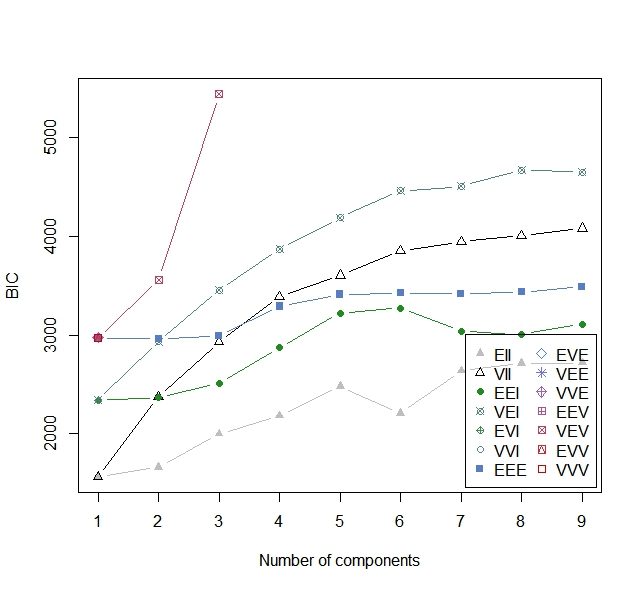
\includegraphics[width=8cm]{BIC}\\
  \caption{The Bayesian Information Criterion. A large BIC score indicates strong evidence for the corresponding model.}\label{BIC}
\end{figure}

Also, the average silhouette method for the hierarchical cluster suggests a model with 3 components (Figure \ref{silHC}). It measures the quality of a clustering, determining how well each object lies within its cluster. A high average silhouette width indicates a good clustering. This method computes the average silhouette of observations for different possible numbers of cluster ($k$). The optimal number of clusters $k$ is the one that maximize the average silhouette over a range of possible values for k (Kaufman and Rousseeuw [1990]).

\begin{figure}[h]
  \centering
    \includegraphics[width=8cm]{silhouetteHC}\\
  \caption{Average Silhouette for Hierarchical clustering}\label{silHC}
\end{figure}


\begin{figure}[h]
  \centering
    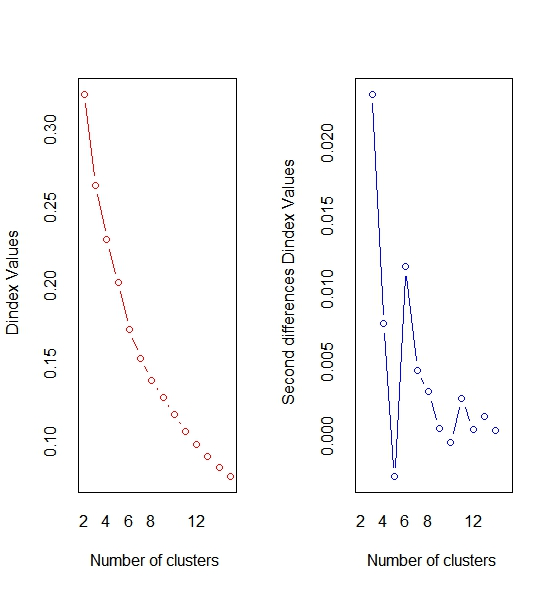
\includegraphics[width=8cm]{NbClust}\\
  \caption{The Dindex}\label{NbClust}
\end{figure}
Finally we run the R. (cran Project) Nbclust function that computes an high number of indices for cluster validation. According to the majority rule, the best number of clusters suggested by Nclust is 3, with 7 indices suggesting that model. In the plot of D index (Figure\ref {NbClust}), we seek a significant knee (the significant peak in Dindex second differences plot) that corresponds to a significant increase of the value of the measure.

As results all three methods suggest a model with 3 component. Among them, we choose to use the classification suggested by the Nbclust method. INSERIAMO UNA TABELLA CON LA CLASSIFICAZIONE?

\subsubsection{Rough set features selection}
This phase aims to find a subset of features which have the same quality as the complete feature set. In other words, the purpose of the rough set feature selection method is to select the significant features and eliminate the not relevant ones.
We use this method to find the socioeconomic features that are useful for the classification of tourists in respect to the cluster families (previous step).
\textcolor{red}{SPIEGO COME LAVORA LA rough SET ANALYSIS?}

So, starting from the knowledge of $Y$ we select the rough set of elements $\in A$
\begin{equation}
A=\{gender,age,country,level of study,profession,willingness to pay\}
\end{equation}

The final rough set eliminated the $level of study$ feature from $A$, creating a feature subset of 6 attributes $Y$:
\begin{equation}
A^1=\{gender,age, country,profession,willingness to pay\}
\end{equation}

\subsection{Cluster Analysis}
In this phase we did a cluster analysis of the max and medium values of utilities (COME LE CHIAMO?) together with the socioeconomic $A^1$ data in order to find homogeneous groups of people that value in the same manner the space. Especially, groups of people that give the same importance to spend time in particular places of the Alghero's territory.

SPIEGARE IL METODO gower USATO PER DETERMINARE LE DISTANZE DI VALORI CATEGORICI


\subsubsection{Hierarchical cluster}

We did a first cluster analysis with the hierarchical method using Ward classification.
SPIEGARE IN COSA CONSISTE IL METODO WARD E PERCHè è FRA I MIGLIORI.

Results show a dendrogram with 5 distinct cluster as suggested by the silhouette widt X (Figure \ref{hcW} and Figure \ref{grW5}).
COMMENTARE I RISULTATI E MOSTRARE UNA SINTESI DEI CLUSTER E DELLE LORO CARATTERISTICHE. FARE GRAFICI DI SINTESI DELLE CARATTERISTICHE PERSONALI E DISEGNO DELLE FUNZIONI DI UTILITà.

\begin{figure}[h]
  \centering
    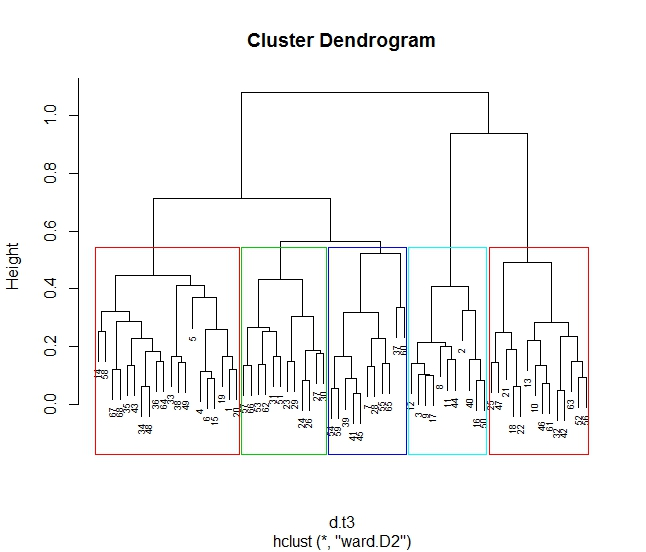
\includegraphics[width=9cm]{hc_Ward_5}\\
  \caption{Dendrogram}\label{hcW}
\end{figure}

\begin{figure}[h]
  \centering
    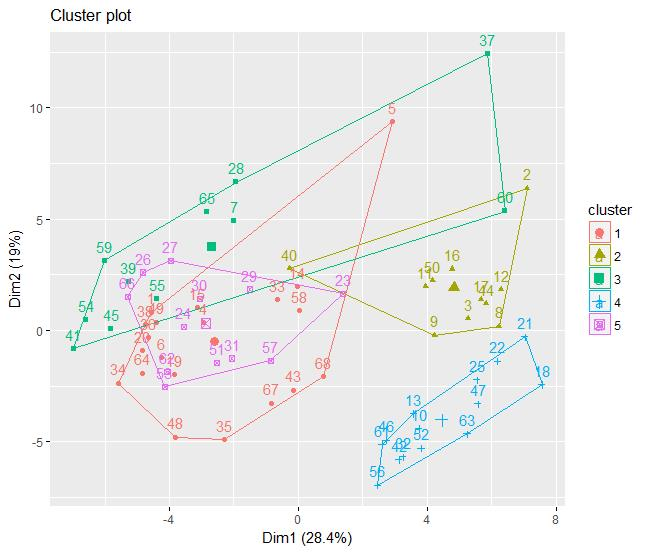
\includegraphics[width=9cm]{grW5}\\
  \caption{Dendrogram}\label{grW5}
\end{figure}

The resulting clusters show different compositions of individuals and of preferences.
\begin{figure}[h]
  \centering
    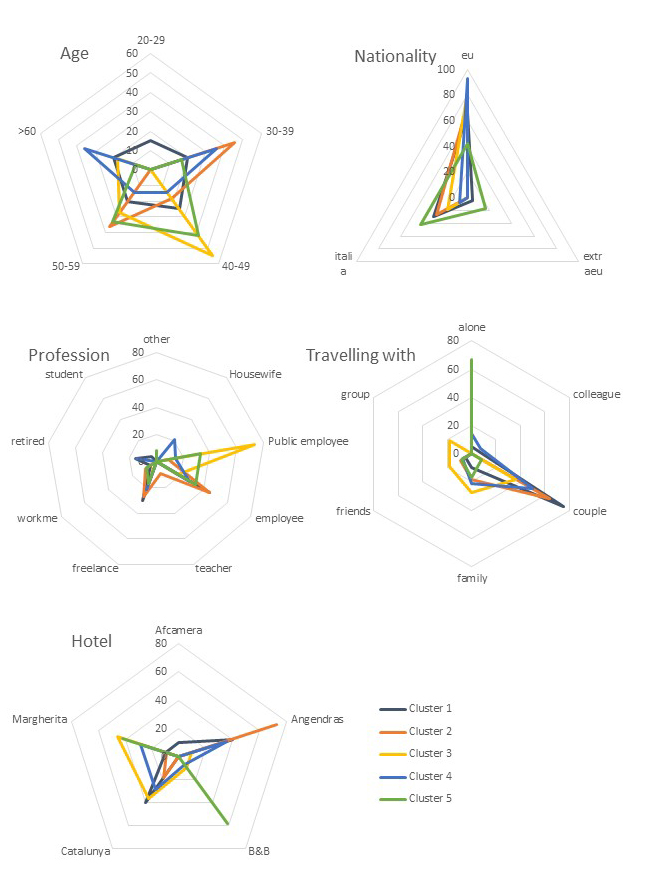
\includegraphics[width=\textwidth]{grafici1}\\
  \caption{Personal Characteristics}\label{gr1}
\end{figure}

\begin{figure}[h]
  \centering
    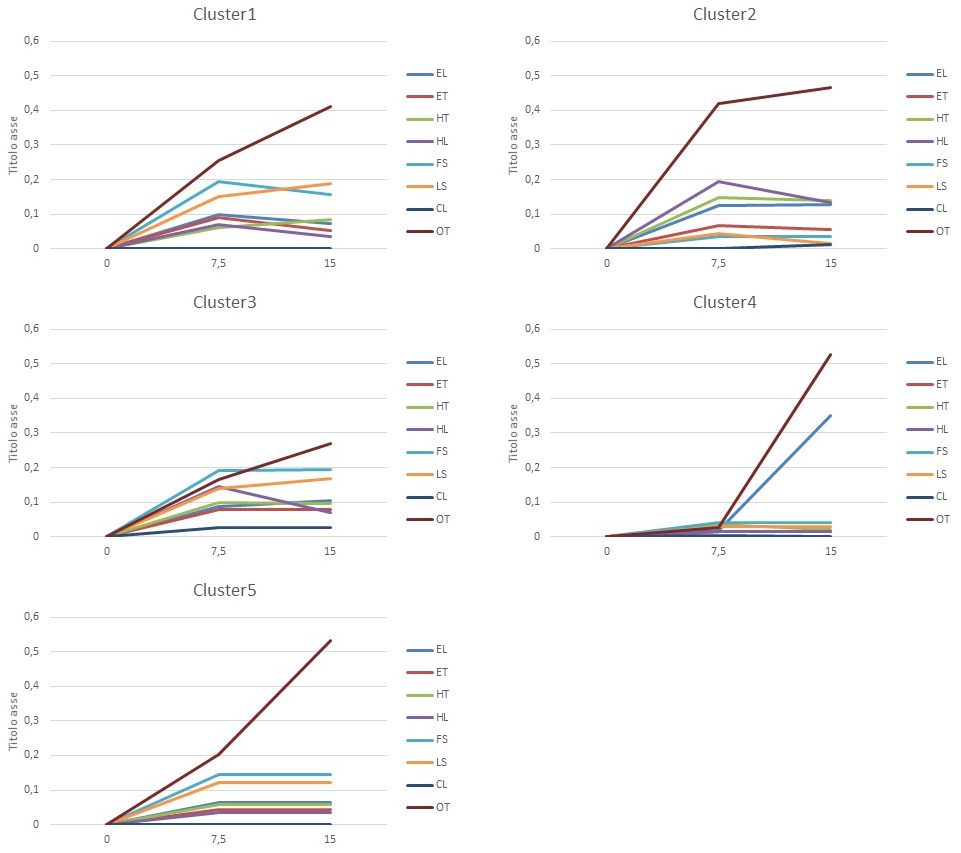
\includegraphics[width=\textwidth]{grafici2}\\
  \caption{Utility Functions}\label{gr2}
\end{figure}


\subsection{pam}
DESCRIVIAMO ANCHE QUESTI RISULTATI? IL MODELLO MIGLIORE è QUELLO CON HIERARCHICAL ANALYSIS MA POSSIAMO MOSTRARE ACHE QUESTI RISULTATI CHE MOSTRANO UNA SUDDIVISIONE IDEALE DI 8 CLUSTER. iL METODO DI SUDDIVISIONE è DIVERSO DAL PRECEDENTE, PER QUESTO RESTITUISCE RISULTATI DIVERSI. (see the word document)


\subsection{A multicriteria recommender system?}
A partire da questi dati trovare un modo per:
\begin{itemize}
\item{vautare l'opportunità di una azione o politica rispetto alle funzioni di utilità dei miei turisti}
\item{generare nuove politiche a partire dall'analisidella differenza tra domanda e offerta}
\item{e se volessi cambiare i turisti?}
\end{itemize}

\subsection{some tests}

\begin{itemize}
    \item\textbf{test1}: Fare una analisi di regressione multipla per definire la relazione tra i risultati ottenuti con la cluster analysis e le componenti socioeconomiche (HO FATTO ALCUNI TEST, DA VERIFICARE CON OLIVIER)
     \item\textbf{test2}:  Multirating collaborative filtering? non so se posso usarla con dati misti ma provo a studiare la questione.
     \item\textbf{test3}: Analisi di regressione tra le preferenze dichiarate e le utilità.

    \end{itemize}

\subsection{Recommendation}



\bibliographystyle{plain}
\bibliography{mybibfile}



\section{Appendix}

\begin{table}[h]
\centering
\begin{tabular}{rrrrrrrrrr}
  \hline
&Test&wEL&wET&wHT&wHL&wFS&wLS&wCL&wOT \\
\parbox{4cm}{range 0-max +20perc}&t1&0,000&0,000&0,000&0,000&0,000&0,000&0,000&1,000 \\
\parbox{4cm}{range automatico}&t2&0,155&0,155&0,097&0,117&0,000&0,155&0,000&0,321 \\
\parbox{4cm}{range(0-max+20perc)+ideal}&t3&0,000&0,048&0,217&0,000&0,086&0,000&0,213&0,437 \\
\parbox{4cm}{range automatico+ideal}&t4&0,155&0,155&0,097&0,117&0,000&0,155&0,000&0,321 \\
\parbox{4cm}{(0-54000)+ideal e antiideal}&t5&0,160&0,145&0,218&0,000&0,000&0,226&0,000&0,252 \\
\parbox{4cm}{(0-54000)+6 alternative+preferenze fra alternative}&t6&0,140&0,129&0,150&0,051&0,000&0,167&0,000&0,363 \\
\parbox{4cm}{(0-54000)+7 alternative+preferenze fra alternative}&t7&0,106&0,097&0,086&0,119&0,197&0,137&0,000&0,259 \\
\parbox{4cm}{(0-54000)+8 alternative+preferenze fra alternative}&t8&0,103&0,109&0,124&0,093&0,067&0,089&0,183&0,231 \\
\parbox{4cm}{(0-54000)+9 alternative+preferenze fra alternative}&t9&0,105&0,106&0,115&0,098&0,104&0,105&0,128&0,240 \\
\parbox{4cm}{(0-54000)+10 alternative+preferenze fra alternative}&t10&0,075&0,065&0,081&0,046&0,211&0,142&0,000&0,379 \\
\parbox{4cm}{(0-54000)+18 alternative+preferenze fra alternative}&t11&0,118&0,118&0,118&0,118&0,118&0,118&0,118&0,172 \\
\parbox{4cm}{(0-54000)-10 alternative utilità - 18alternative conferma utilità}&t12&0,125&0,125&0,125&0,125&0,125&0,125&0,125&0,125 \\
\parbox{4cm}{(0-54000)-10 alternative utilità - 18 alternative conferma utilità}&t13&0,075&0,065&0,081&0,046&0,211&0,142&0,000&0,379 \\
\hline
\end{tabular}
\caption{\textbf{all Test}}\
\label{Table4}
\end{table}

\end{document}

